\section{DDNS}
Um immer die aktuelle IP-Adresse des Pi zur Hand zu haben, wurde ein DynDNS-Client von no-ip implementiert, bei jedem Systemstart wird die bei der DNS hinterlegte IP-Adresse aktualisiert.\\
Nachteil hierbei ist jedoch, dass man alle 30 Tage diese Domain aktivieren muss, da diese sonst verfällt.\\
Um dies zu umgehen wurde die Kostenfreie Domain bananapihfu.tk gebucht. Von Vorteil ist hier, dass diese Domain eine Laufzeit von einem Jahr hat und nach Ablauf auch ohne Mehrkosten verlängert werden kann.\\
Diese Domain wird bei Cloudflare verwaltet, da hier auch eine API angeboten wird, mit welcher man Theoretisch komplett auf eine Dynamische DNS bei No-IP verzichten kann.

\subsection{Einrichtung No-IP}
Voraussetzungen:\\
- Internetzugriff\\
- SSH/Physikalischen Zugriff\\
- NoIP.com Account\\
\\
1. NoIP Hostnamen anlegen:\\
Man muss in No-IP den gewünschten Hostnamen einrichten, welcher später auf die aktuelle IP-Adresse verweist.\\
\begin{figure}[ht]
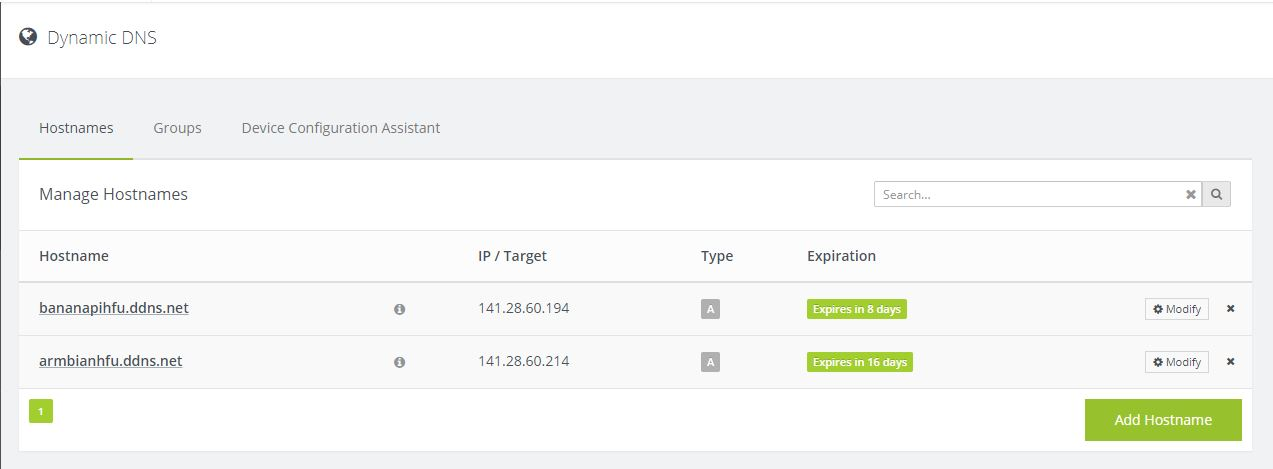
\includegraphics[width=\textwidth]{pictures/Jonas/noip_Domain}
\caption{noip Domain}
\end{figure}
~\\
2. Verzeichnis für DDNS im Homeverzeichnis erstellen und wechseln:
\begin{lstlisting}
mkdir DDNS
cd DDNS
\end{lstlisting}
~\\
3. NoIP-Client von NoIP.com beziehen:
\begin{lstlisting}
wget https://www.noip.com/client/linux/noip-duc-linux.tar.gz
\end{lstlisting}
~\\
4. Das Archiv entpacken:
\begin{lstlisting}
tar xvf noip-duc-linux.tar.gz
\end{lstlisting}
~\\
5. In den Entpackten Ordner wechseln:\\
cd noip eingeben und mit TAB vervollständigen
\begin{lstlisting}
cd noip-x.x.x-x 
\end{lstlisting}
~\\
6. Client bauen und installieren:
\begin{lstlisting}
make && make install
\end{lstlisting}
~\\
7. Konfiguration wird gestartet:
\begin{figure}[ht]
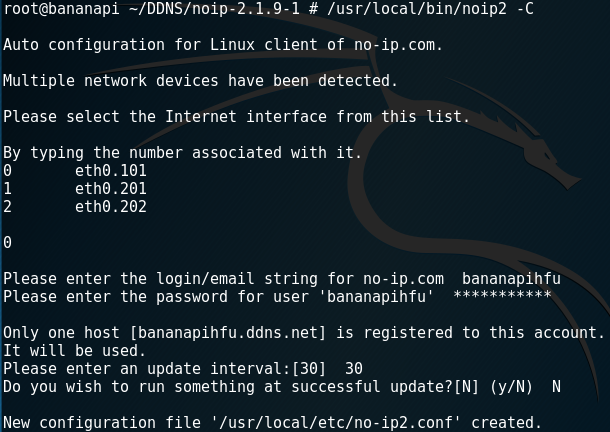
\includegraphics[width=\textwidth]{pictures/Jonas/noip_Konfiguration}
\caption{noip Konfiguration}
\end{figure}

~\\
Um den Daemon automatisch bei Systemstart zu starten muss noch folgende Konfiguration vorgenommen werden:\\
1. Startscript unter /etc/init.d/noip2 ablegen:
\begin{lstlisting}
vim /etc/init.d/noip2
\end{lstlisting}
~\\
2. Script "noip2" kopieren und einfügen:\\
Verweis auf Anhang\\
~\\
3. Script ausführbar machen:
\begin{lstlisting}
chmod a+rx /etc/init.d/noip2
\end{lstlisting}
~\\ Quelle: https://www.togaware.com/linux/survivor/No\_IP\_Manual.html \cite{noip}
\newpage
\subsection{Einrichtung Custom-Domain}
Voraussetzungen:\\
- Account bei Cloudflare\\
~\\
1. Domain bei Freenom.com aussuchen:\\
Hier gibt es jede Menge kostenfreie Domains\\
~\\
2. Wunsch-Domain registrieren\\
\begin{figure}[ht]
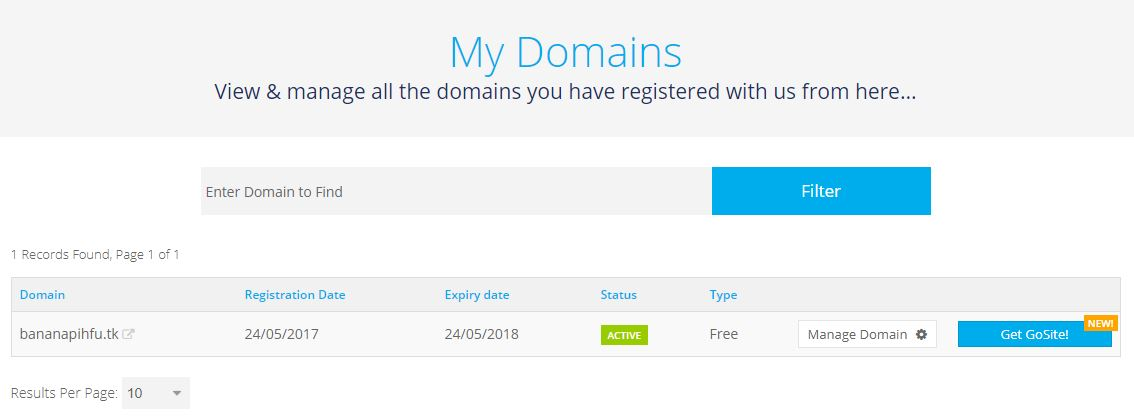
\includegraphics[width=\textwidth]{pictures/Jonas/freenom_Domain}
\caption{freenom Domain}
\end{figure}

3. Nameserver bei Freenom ändern:\\
Um die Domain bei Cloudflare zu verwalten, müssen die Nameserver angepasst werden.
Diese erhält man, wenn man sich bei Cloudflare anmeldet.\\
\begin{figure}[ht]
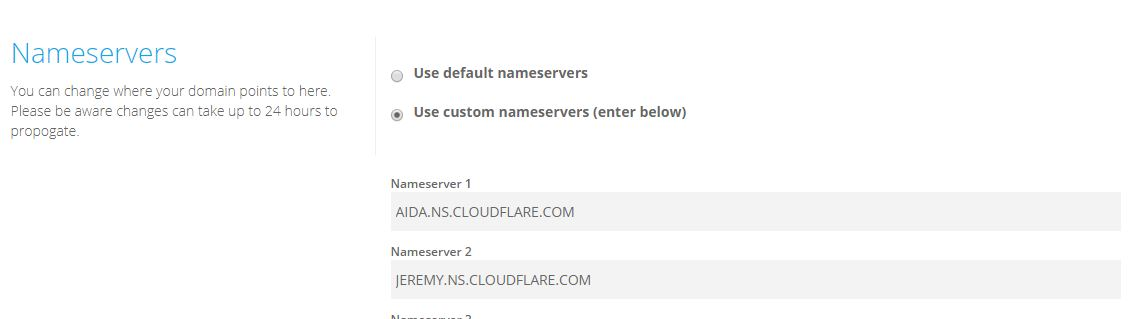
\includegraphics[width=\textwidth]{pictures/Jonas/freenom_Nameserver}
\caption{freenom Nameserver}
\end{figure}
\newpage
3. CNAME Weiterleitung auf No-Ip einrichten\\
\begin{figure}[ht]
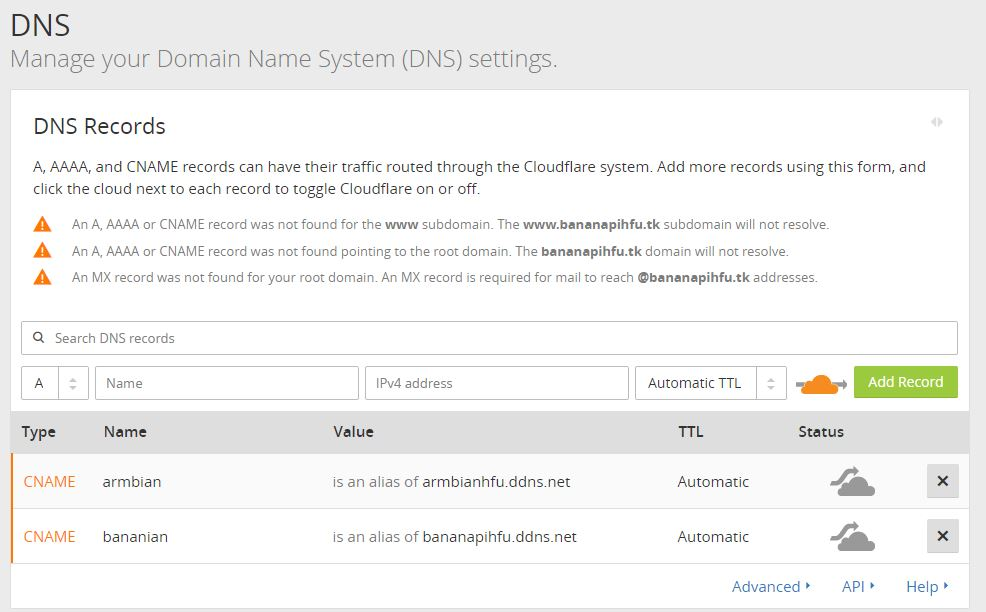
\includegraphics[width=\textwidth]{pictures/Jonas/Cloudflare_DNS}
\caption{Cloudflare DNS}
\end{figure}


